\subsection{Tiempo de uso promedio de los usuarios}

En base a los campos Inicio\_del\_viaje y Fin\_del\_viaje se calculo el tiempo de uso de una bicicleta en minutos. Con estos datos se usaron las ecuaciones \ref{eq:monthly_hourly_mean}, \ref{eq:monthly_hourly_var}, \ref{eq:daily_hourly_mean} y \ref{eq:daily_hourly_var}. Los resultados obtenidos son los siguientes:

\subsubsection{Promedio y desviación estandar mensual por hora}

En la figura \ref{fig:monthly_hourly_mean_time} se visualiza que existe un aumento en el tiempo de uso entre los meses octubre y diciembre. Este último coincide con el fin de la temporada con más frecuencia de lluvias y una disminución de la temperatura\cite{clima_guadalajara}.

\begin{figure}[H]
    \centering
    \begin{subfigure}[b]{8cm}
        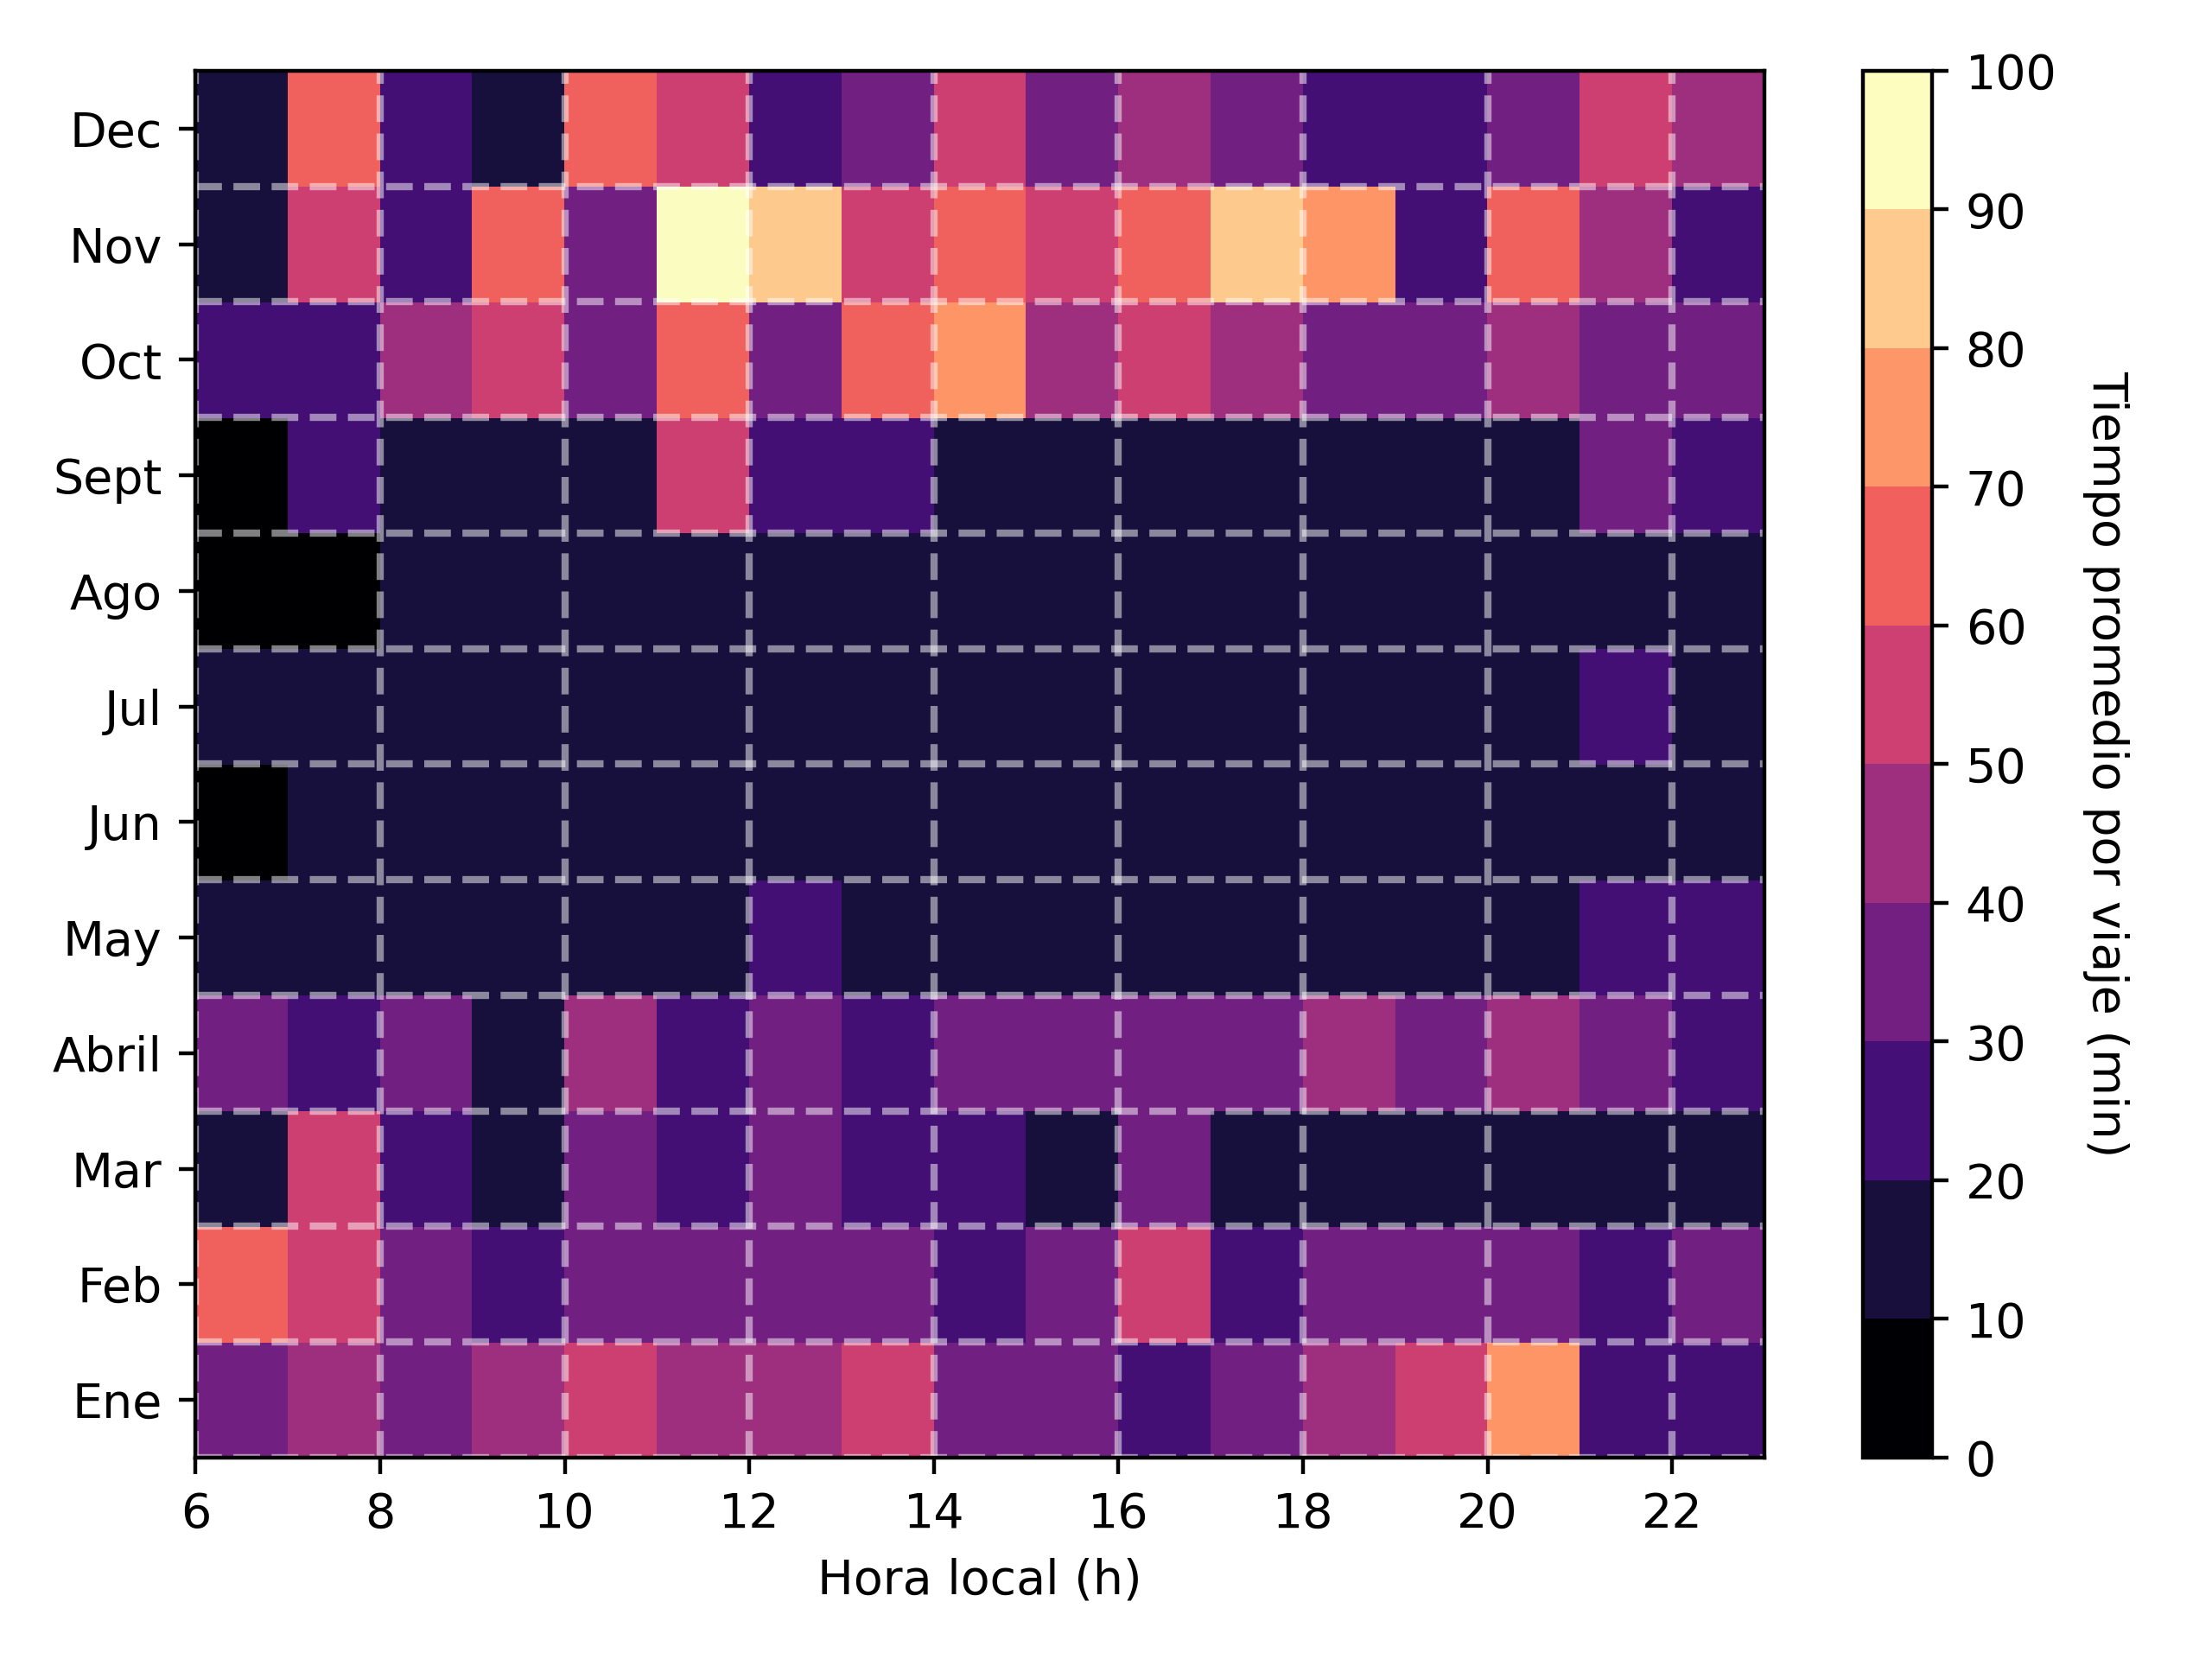
\includegraphics[width=8cm]{Graphics/monthly_hourly_mean_time_travel.png}
        \caption{Promedio mensual del tiempo de uso.}
        \label{fig:monthly_hourly_mean_time}
    \end{subfigure}
    \begin{subfigure}[b]{8cm}
        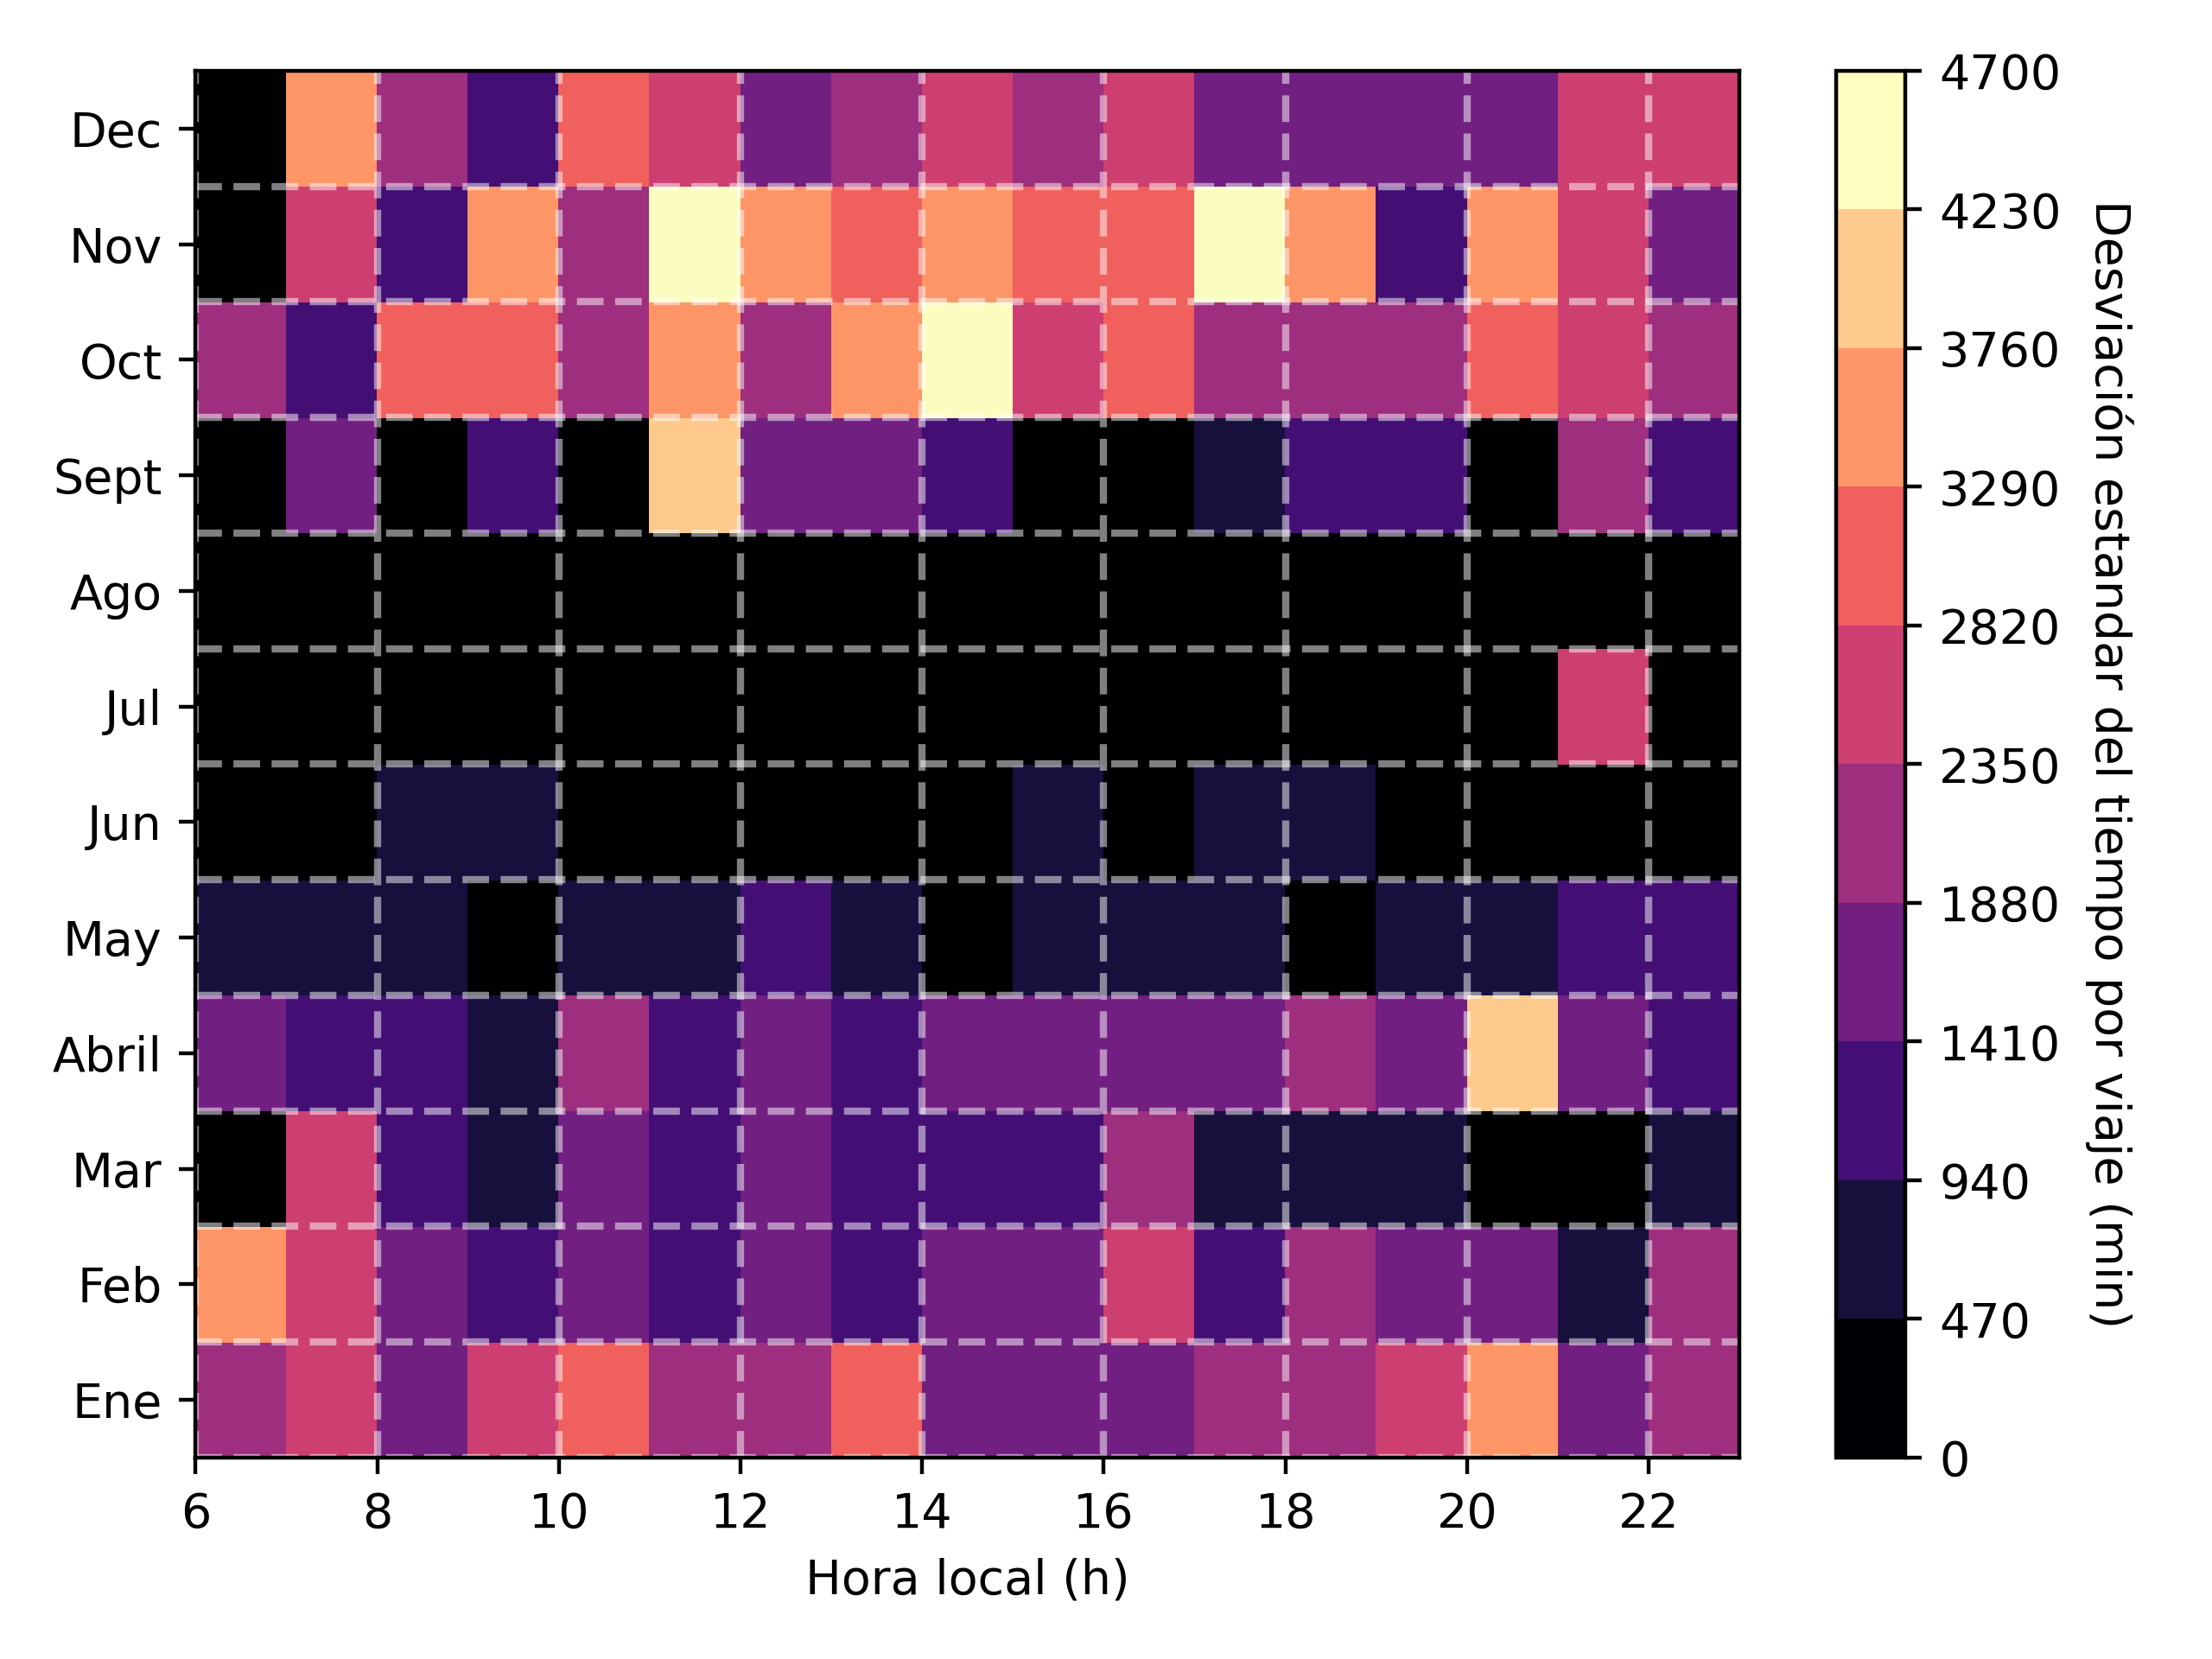
\includegraphics[width=8cm]{Graphics/monthly_hourly_var_time_travel.png}
        \caption{Desviación estandar del tiempo de uso.}
        \label{fig:monthly_hourly_var_time}
    \end{subfigure}
    \caption{Tiempo de uso promedio y desviación estandar mensual por hora de lo usuarios calculadas con las ecuaciones \ref{eq:monthly_hourly_mean} y \ref{eq:monthly_hourly_var}.}
    \label{fig:monthly_hourly_time}
\end{figure}

En la figura \ref{fig:monthly_hourly_mean_time} se presenta un mínimo entre los meses de mayo y agosto. Con ayuda de la figura \ref{fig:monthly_hourly_var_time} se obtiene que el tiempo de uso de los usuarios entre los meses de octubre y diciembre tienen una mayor variación y esto puede deberse a que la baja temperatura y baja probabilidad de lluvia\cite{clima_guadalajara}, ya que algunos usuarios pueden dejar de usarlas al sentir una incomodidad y otros prefieran usar más el servicio. Además, los usuarios pueden sentir menos preocupación de las vías públicas y el usar la bicicleta representa más un momento de descanso de su rutina.

\subsubsection{Promedio y desviación estandar diaria semanal por hora}

En la figura \ref{fig:daily_hourly_time} se aprecia que no hay alguna preferencia en los tiempos de uso en los dias entre semana, por lo que se podria estimar un tiempo promedio de uso para toda la semana.

El factor más importante a tomar en cuenta es el mes del que se trate, ya que como se describió en la figura \ref{fig:monthly_hourly_time}, sí existen variaciones a lo largo del año. En la figura \ref{fig:daily_hourly_var_time} entre las 8 y 10 am se ve que existe una mayor variación en el tiempo de uso. Lo cual concuerda con lo antes mencionado en la figura \ref{fig:daily_hourly_var_distance}

\begin{figure}[H]
    \centering
    \begin{subfigure}[b]{8cm}
        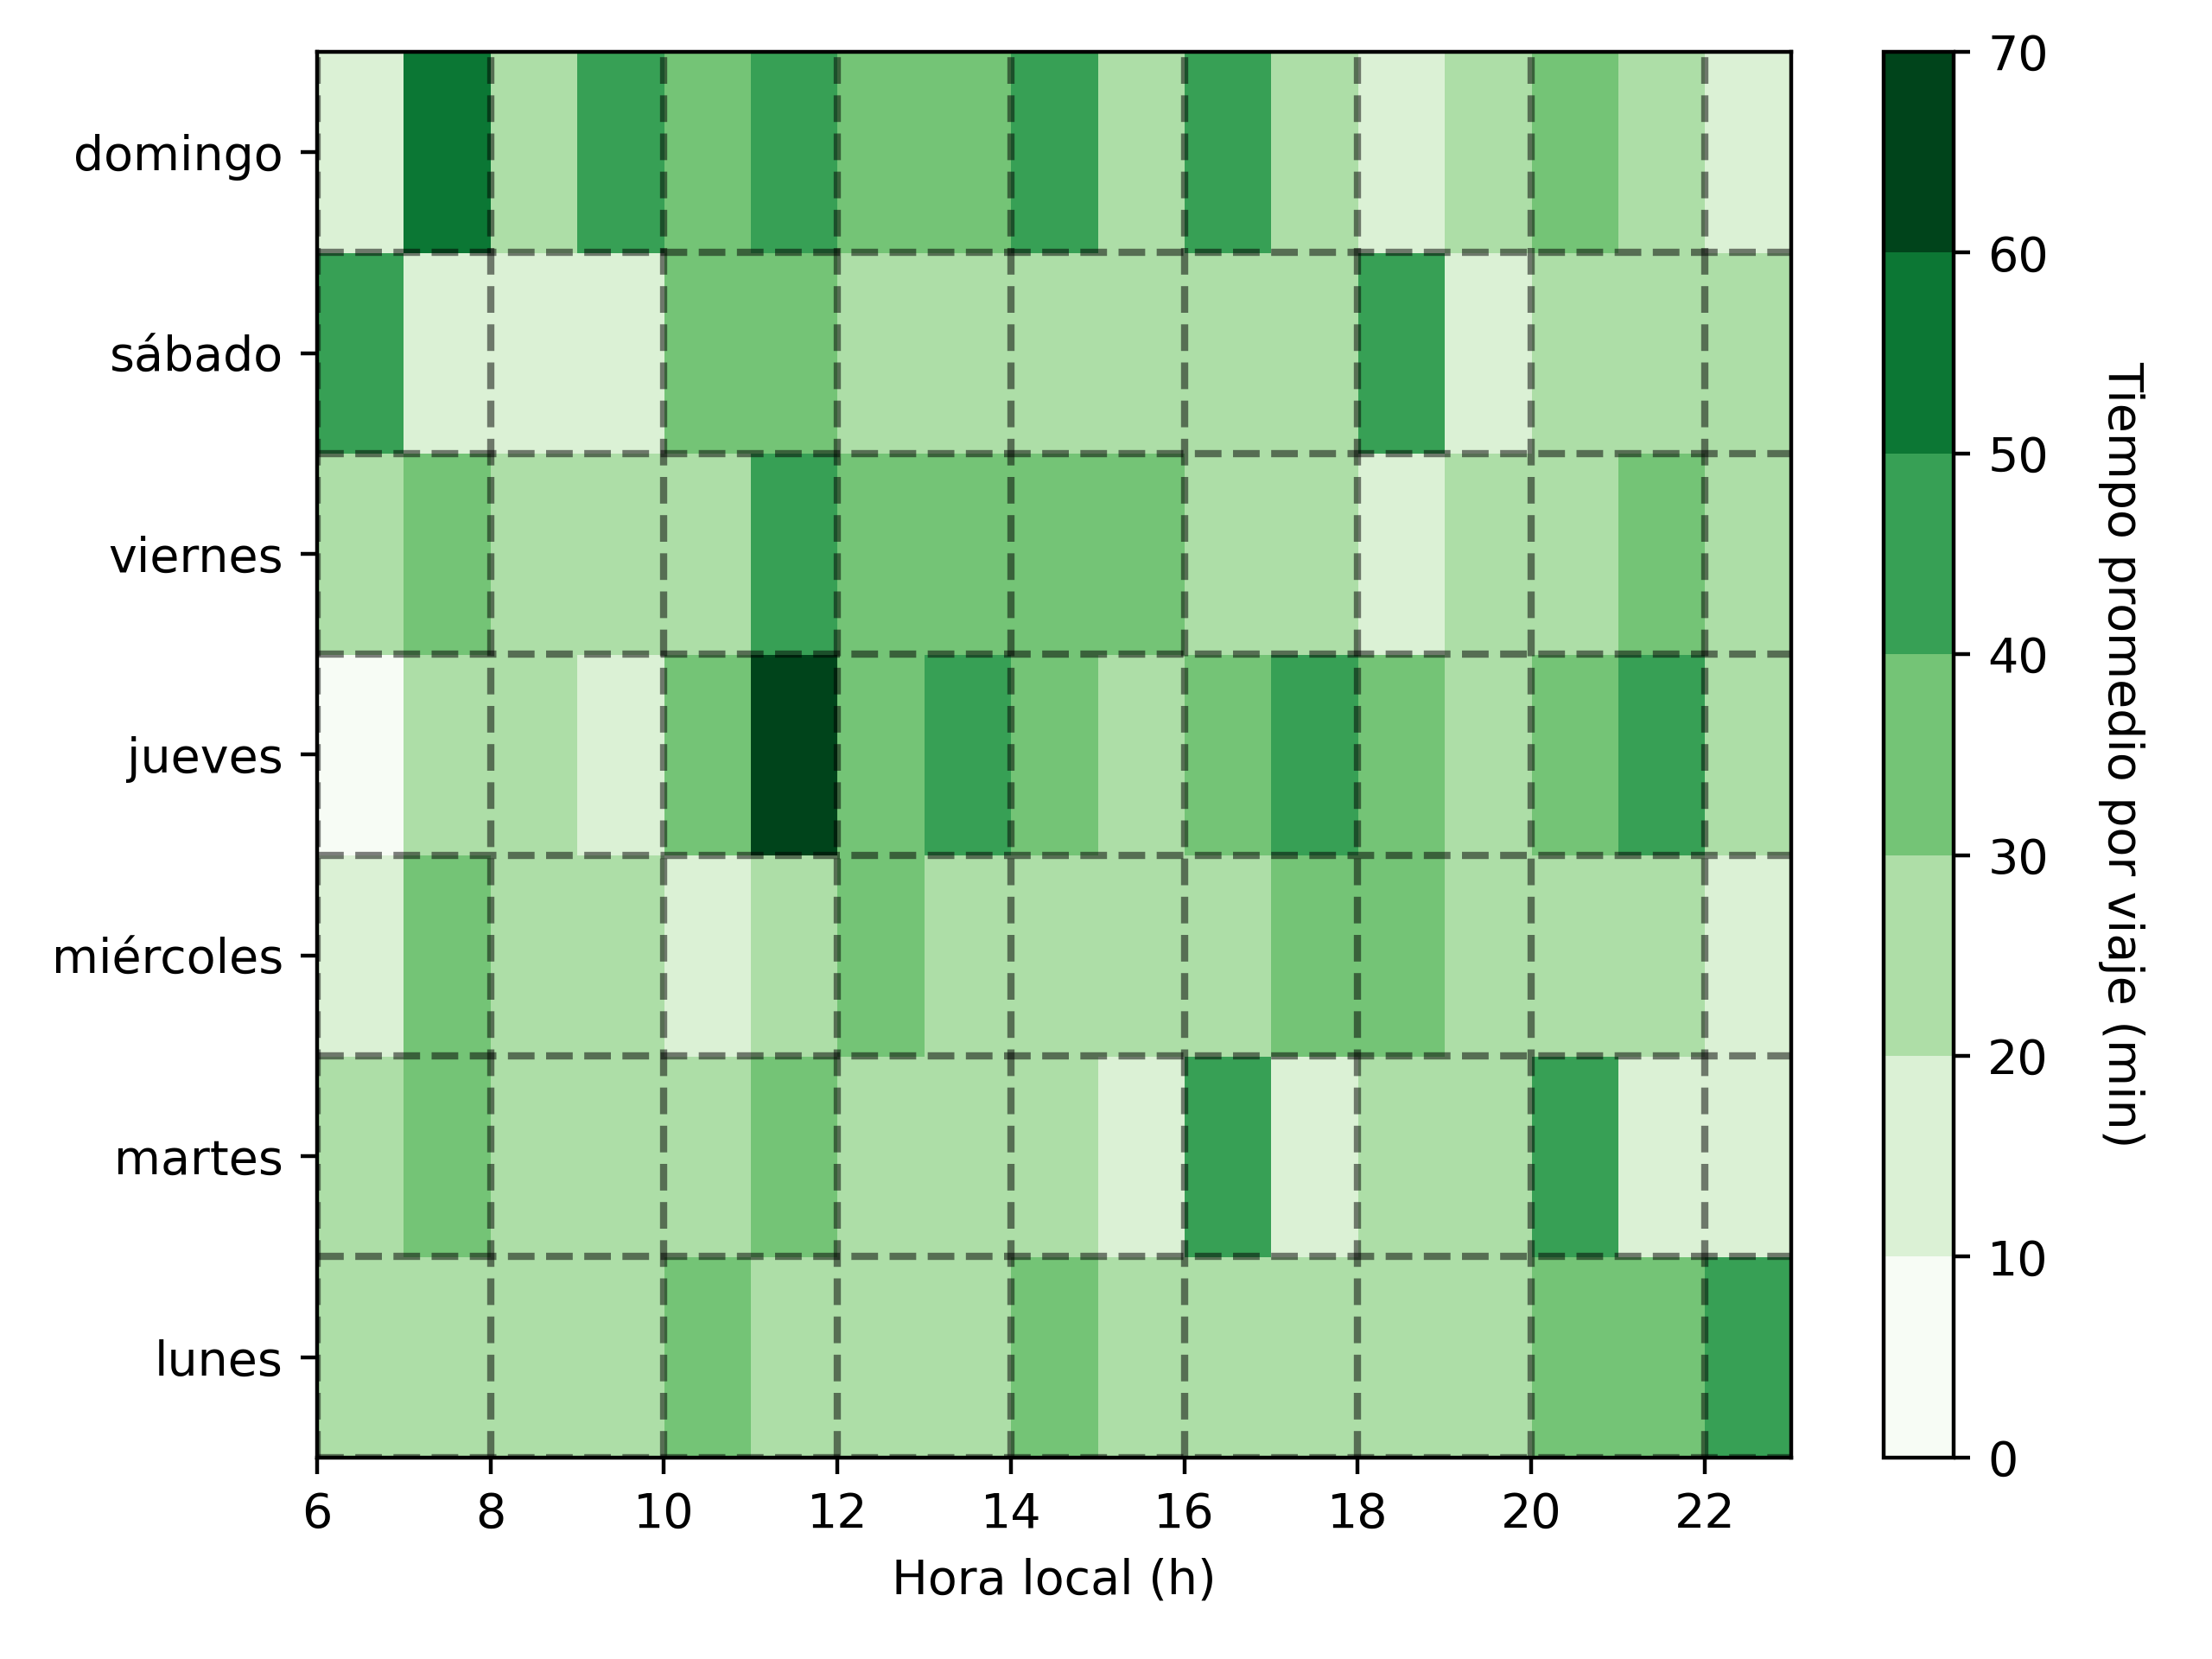
\includegraphics[width=8cm]{Graphics/daily_hourly_mean_time_travel.png}
        \caption{Promedio diario semanal.}
        \label{fig:daily_hourly_mean_time}
    \end{subfigure}
    \begin{subfigure}[b]{8cm}
        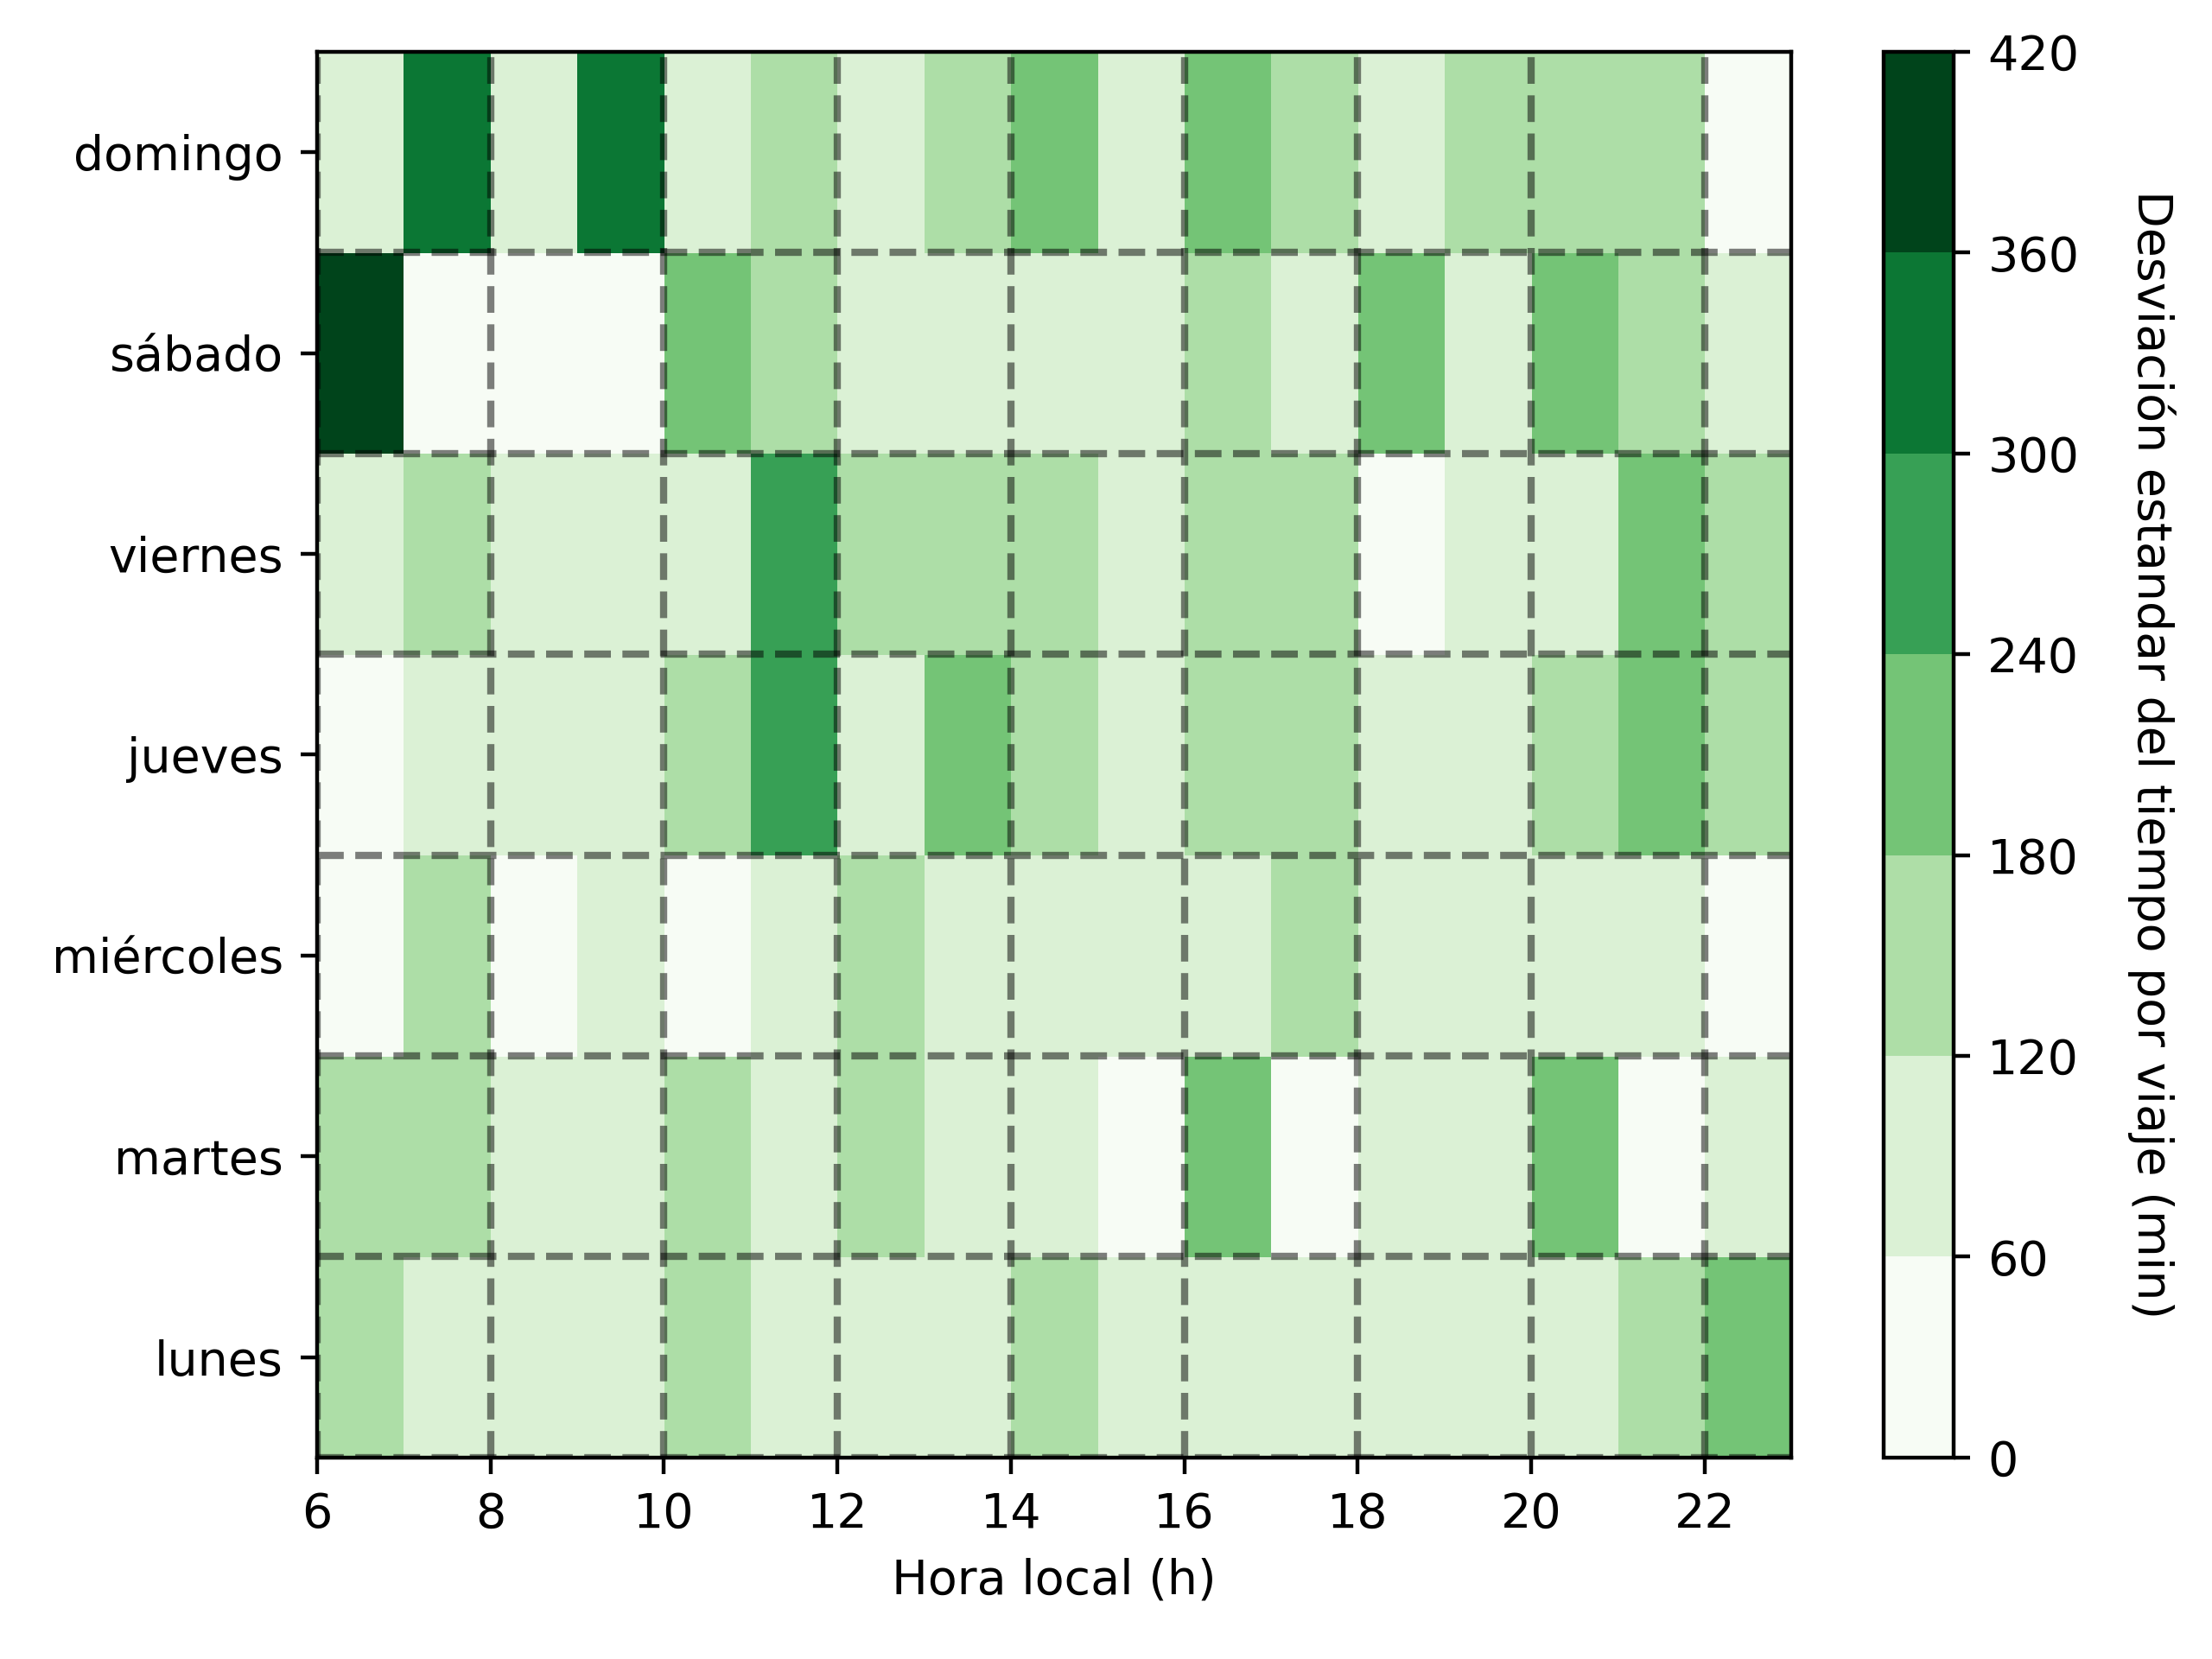
\includegraphics[width=8cm]{Graphics/daily_hourly_var_time_travel.png}
        \caption{Desviación estandar diaria semanal.}
        \label{fig:daily_hourly_var_time}
    \end{subfigure}
    \caption{Tiempo de uso promedio y desviación estandar diaria semanal por hora de los usuarios calculadas con las ecuaciones \ref{eq:daily_hourly_mean} y \ref{eq:daily_hourly_var}.}
    \label{fig:daily_hourly_time}
\end{figure}

\subsubsection{Distribución del tiempo de uso de una bicicleta}

A partir de los tiempos calculados para todos los viajes realizados en el periodo 2015-2018 se usó la ecuación \ref{eq:hourly_mean}. La distribución de estos datos se muestran en la figura \ref{fig:distribution_times}. Aqui se observa como la correspondencia de la figura \ref{fig:distribution_distances} se ve representada en los tiempos de uso. Ya que al recorrer una misma distancia esta tiene un tiempo semejante cada vez que se realiza.

\begin{figure}[H]
    \centering
    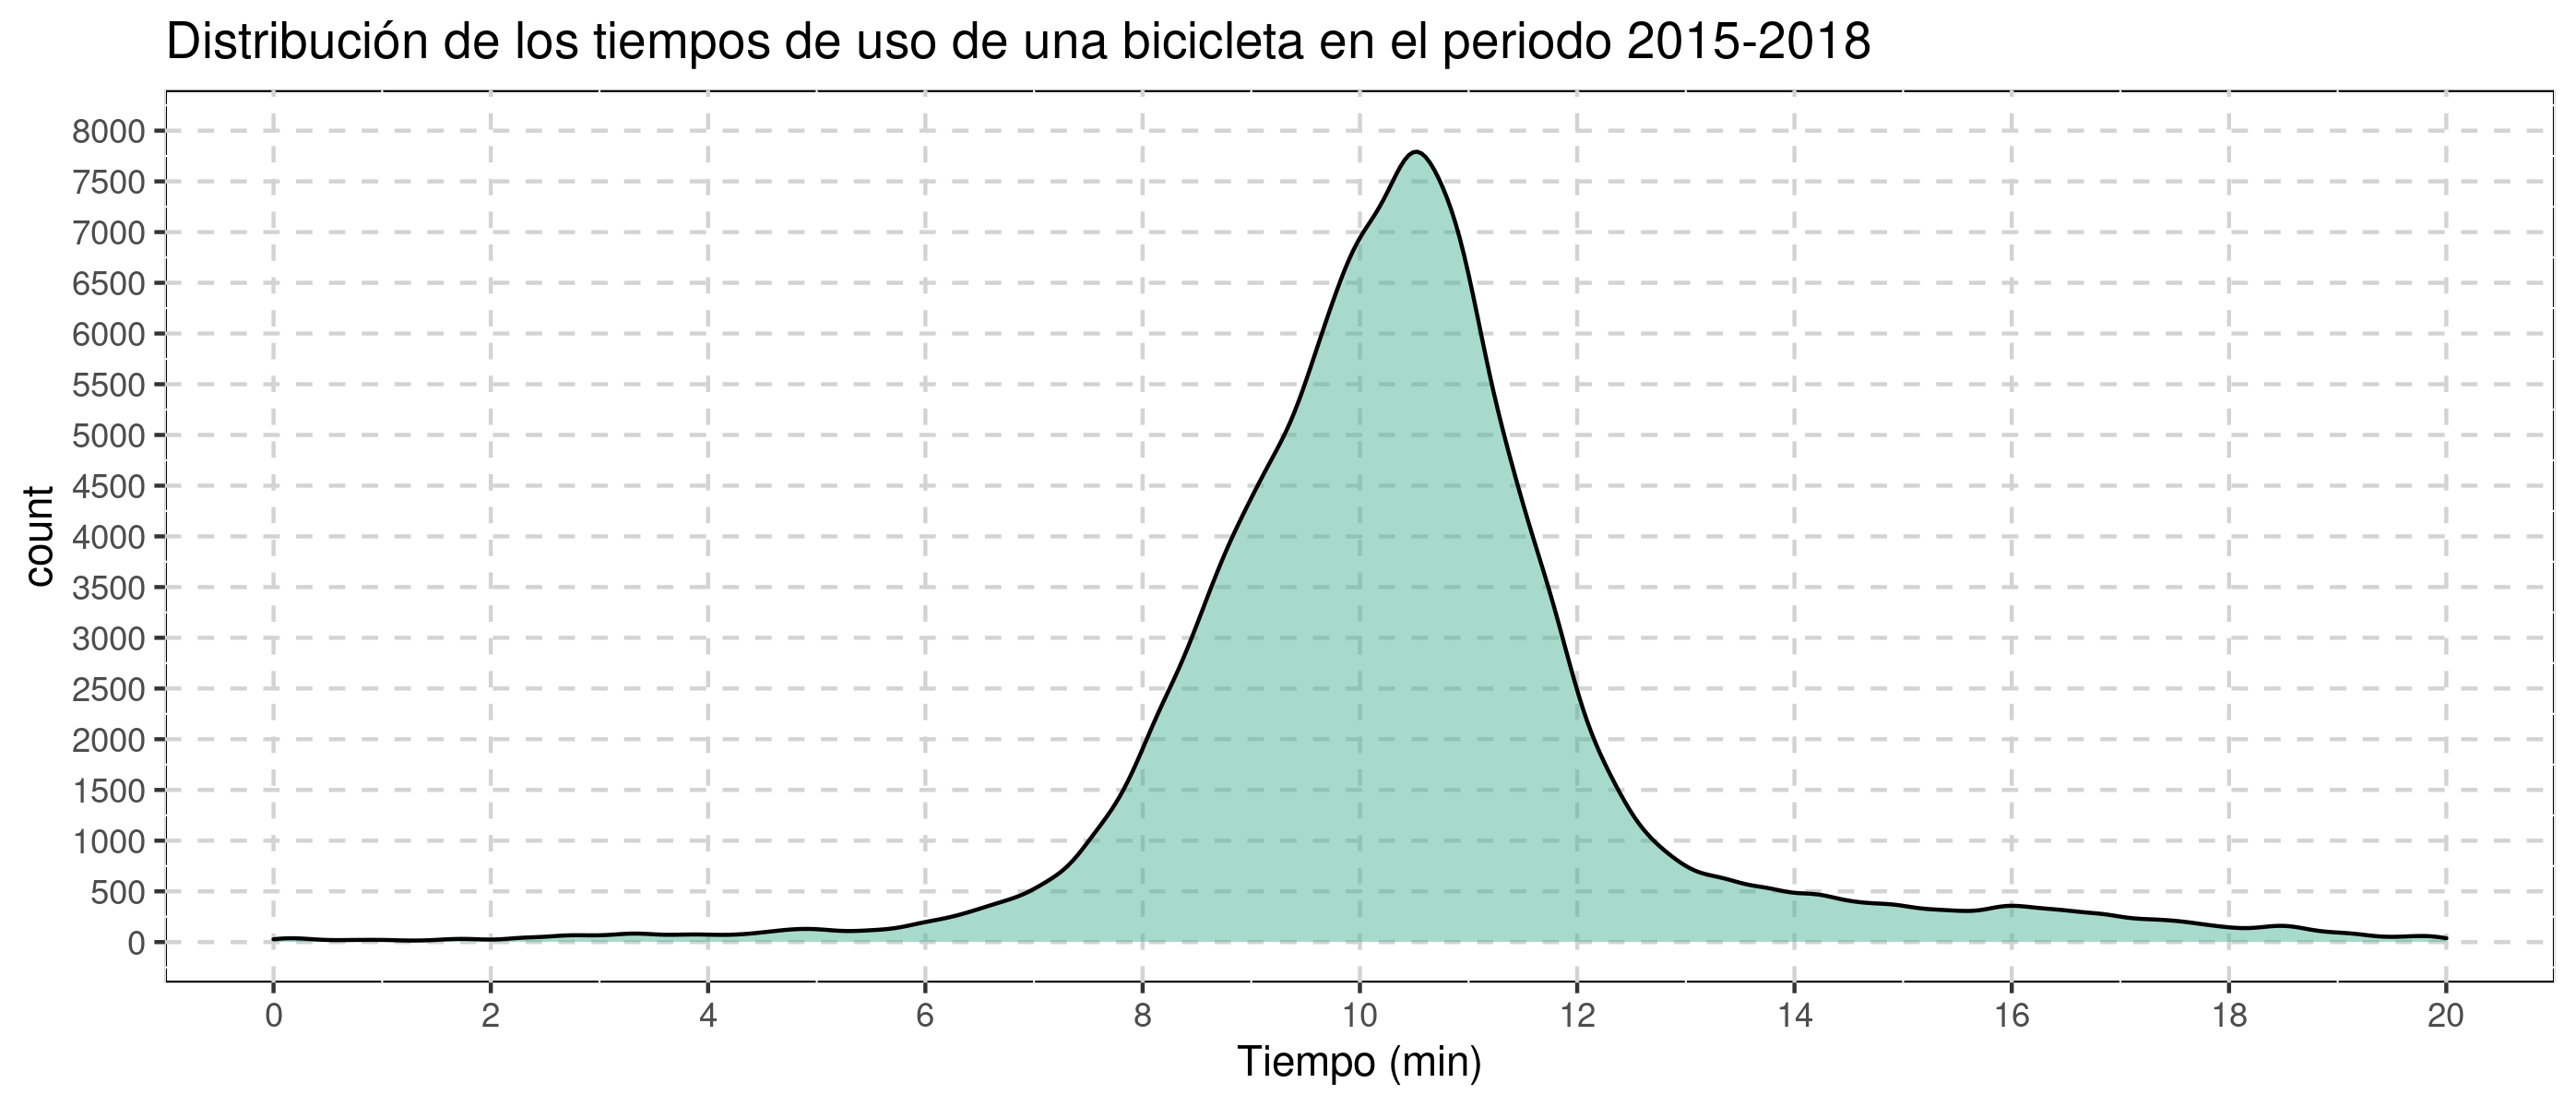
\includegraphics[width=16cm]{Graphics/distribution_time_travel.png}
    \caption{Distribución del tiempo de uso de una bicicleta en el periodo 2015-2018.}
    \label{fig:distribution_times}
\end{figure}